% answers.tex —— 2010 年·普通高等学校招生考试·上海卷·文科 · 参考答案与详细解析片段
% 由 tools/generate_projects.py 依来源总账自 2010/2010_数学真题_上海文_试题.md + 2010/2010_数学真题_上海文_解析正文.md + 2010/2010_数学真题_上海文_答案要点.md 生成，勿手改（改源 MD 后重跑）


\begin{gktip}
固定候选 PDF 仅含题面，无答案、解析和评分标准，原页亦未标分值；以下为非官方编者独立推导，官方答案字段为空。分数、根号、上下标与两幅图均以 600 dpi 原页复核。
\end{gktip}

\begin{answer}
\gksolhead{1}{}

\textbf{题目}：

已知集合 $A=\{1,3,m\}$，$B=\{3,4\}$，$A\cup B=\{1,2,3,4\}$，则 $m=$ $\underline{\qquad}$．

\Needspace{4\baselineskip}
\textbf{解析}

$A\cup B=\{1,3,m,4\}=\{1,2,3,4\}$，故 $m=2$。

\gkanswer{答案：$2$。}

\end{answer}
\begin{answer}
\gksolhead{2}{}

\textbf{题目}：

不等式 $\dfrac{2-x}{x+4}>0$ 的解集是$\underline{\qquad}$．

\Needspace{4\baselineskip}
\textbf{解析}

$\dfrac{2-x}{x+4}>0$ 等价于 $(x-2)(x+4)<0$，故 $-4<x<2$。

\gkanswer{答案：$(-4,2)$。}

\end{answer}
\begin{answer}
\gksolhead{3}{}

\textbf{题目}：

行列式 $\begin{vmatrix}\cos\dfrac\pi6&\sin\dfrac\pi6\\ \sin\dfrac\pi6&\cos\dfrac\pi6\end{vmatrix}$ 的值是$\underline{\qquad}$．

\Needspace{4\baselineskip}
\textbf{解析}

\Needspace{5\baselineskip}
推导如下。

\nopagebreak[4]
\[\begin{vmatrix}\cos\frac\pi6&\sin\frac\pi6\\ \sin\frac\pi6&\cos\frac\pi6\end{vmatrix}
=\cos^2\frac\pi6-\sin^2\frac\pi6=\cos\frac\pi3=\frac12.\]

\gkanswer{答案：$\dfrac12$。}

\end{answer}
\begin{answer}
\gksolhead{4}{}

\textbf{题目}：

若复数 $z=1-2\mathrm i$（$\mathrm i$ 为虚数单位），则 $z\cdot\overline z+z=$ $\underline{\qquad}$．

\Needspace{4\baselineskip}
\textbf{解析}

\Needspace{5\baselineskip}
$z\overline z=|z|^2=1+4=5$，故

\nopagebreak[4]
\[z\overline z+z=5+1-2\mathrm i=6-2\mathrm i.\]

\gkanswer{答案：$6-2\mathrm i$。}

\end{answer}
\begin{answer}
\gksolhead{5}{}

\textbf{题目}：

将一个总体分为 $A$、$B$、$C$ 三层，其个体数之比为 $5:3:2$．若用分层抽样方法抽取容量为 $100$ 的样本，则应从 $C$ 层中抽取$\underline{\qquad}$个个体．

\Needspace{4\baselineskip}
\textbf{解析}

\Needspace{5\baselineskip}
$C$ 层占 $\dfrac2{5+3+2}=\dfrac15$，样本中应抽

\nopagebreak[4]
\[100\times\frac15=20.\]

\gkanswer{答案：$20$。}

\end{answer}
\begin{answer}
\gksolhead{6}{}

\textbf{题目}：

已知四棱锥 $P-ABCD$ 的底面是边长为 $6$ 的正方形，侧棱 $PA\perp$ 底面 $ABCD$，且 $PA=8$，则该四棱锥的体积是$\underline{\qquad}$．

\Needspace{4\baselineskip}
\textbf{解析}

\Needspace{5\baselineskip}
底面积 $6^2=36$，高 $PA=8$，

\nopagebreak[4]
\[V=\frac13\cdot36\cdot8=96.\]

\gkanswer{答案：$96$。}

\end{answer}
\begin{answer}
\gksolhead{7}{}

\textbf{题目}：

圆 $C:x^2+y^2-2x-4y+4=0$ 的圆心到直线 $l:3x+4y+4=0$ 的距离 $d=$ $\underline{\qquad}$．

\Needspace{4\baselineskip}
\textbf{解析}

\Needspace{5\baselineskip}
圆化为 $(x-1)^2+(y-2)^2=1$，圆心 $(1,2)$。距离

\nopagebreak[4]
\[d=\frac{|3+8+4|}{\sqrt{3^2+4^2}}=\frac{15}{5}=3.\]

\gkanswer{答案：$3$。}

\end{answer}
\begin{answer}
\gksolhead{8}{}

\textbf{题目}：

动点 $P$ 到点 $F(2,0)$ 的距离与它到直线 $x+2=0$ 的距离相等，则点 $P$ 的轨迹方程为$\underline{\qquad}$．

\Needspace{4\baselineskip}
\textbf{解析}

到焦点 $(2,0)$ 与到准线 $x=-2$ 距离相等，是抛物线 $y^2=2px$，$\dfrac p2=2$，$p=4$，故 $y^2=8x$。

\gkanswer{答案：$y^2=8x$。}

\end{answer}
\begin{answer}
\gksolhead{9}{}

\textbf{题目}：

函数 $f(x)=\log_3(x+3)$ 的反函数的图象与 $y$ 轴的交点坐标是$\underline{\qquad}$．

\Needspace{4\baselineskip}
\textbf{解析}

\Needspace{5\baselineskip}
反函数 $f^{-1}(x)=3^x-3$。令 $x=0$：

\nopagebreak[4]
\[f^{-1}(0)=1-3=-2.\]

\gkanswer{答案：$(0,-2)$。}

\end{answer}
\begin{answer}
\gksolhead{10}{}

\textbf{题目}：

从一副混合后的扑克牌（$52$ 张）中随机抽取 $2$ 张，则“抽出的 $2$ 张均为红桃”的概率为$\underline{\qquad}$．（结果用最简分数表示）

\Needspace{4\baselineskip}
\textbf{解析}

\Needspace{5\baselineskip}
推导如下。

\nopagebreak[4]
\[\frac{\mathrm C_{13}^2}{\mathrm C_{52}^2}
=\frac{78}{1326}=\frac1{17}.\]

\gkanswer{答案：$\dfrac1{17}$。}

\end{answer}
\begin{answer}
\gksolhead{11}{}

\textbf{题目}：

$2010$ 年上海世博会园区每天 $9:00$ 开园，$20:00$ 停止入园．在下边的框图中，$S$ 表示上海世博会官方网站在每个整点报道的入园总人数，$a$ 表示整点报道前 $1$ 个小时内入园人数，则空白的执行框内应填入$\underline{\qquad}$．
\nopagebreak[4]
\begin{center}% 2010 年上海卷文科第 11 题：世博入园人数统计程序框图。
% 来源 PDF：普通高考/2010/2010上海文.pdf，SHA-256 5e81bdb27659512a50968275bf502ee666e2ac3f25f9fcaa1b166576fbe9cf62。
% 原页：第 1 页（A3 三栏）第 1 栏下部，书页码 629。
% 重绘依据：T←9、S←0；输出 T,S；判断 T≤19，是则 T←T+1、输入 a、S←S+a 后回到输出，否则结束。
\begin{tikzpicture}[semithick, every node/.style={inner sep=2pt, font=\small}, >=stealth]
  \node[draw,rounded corners] (start) at (0,0) {开始};
  \node[draw,rectangle] (init) at (0,-1.1) {$T\leftarrow9,\ S\leftarrow0$};
  \node[draw,rectangle] (out) at (0,-2.2) {输出 $T,S$};
  \node[draw,diamond,aspect=2] (test) at (0,-3.5) {$T\leqslant19$};
  \node[draw,rectangle] (inc) at (0,-4.7) {$T\leftarrow T+1$};
  \node[draw,rectangle] (inp) at (0,-5.7) {输入 $a$};
  \node[draw,rectangle] (add) at (0,-6.7) {$S\leftarrow S+a$};
  \node[draw,rounded corners] (end) at (3.2,-3.5) {结束};

  \draw[->] (start) -- (init);
  \draw[->] (init) -- (out);
  \draw[->] (out) -- (test);
  \draw[->] (test) -- node[right] {是} (inc);
  \draw[->] (inc) -- (inp);
  \draw[->] (inp) -- (add);
  \draw[->] (add.east) -- (2.0,-6.7) -- (2.0,-2.2) -- (out.east);
  \draw[->] (test) -- node[above] {否} (end);
\end{tikzpicture}
\end{center}
\nopagebreak[4]
\Needspace{4\baselineskip}
\textbf{解析}

每个整点把前一小时入园人数 $a$ 累加到总人数 $S$。

\gkanswer{答案：$S\leftarrow S+a$。}

\end{answer}
\begin{answer}
\gksolhead{12}{}

\textbf{题目}：

\Needspace{5\baselineskip}
在 $n$ 行 $n$ 列矩阵

\nopagebreak[4]
\[\begin{pmatrix}
1&2&3&\cdots&n-2&n-1&n\\
2&3&4&\cdots&n-1&n&1\\
3&4&5&\cdots&n&1&2\\
\cdots&\cdots&\cdots&\cdots&\cdots&\cdots&\cdots\\
n&1&2&\cdots&n-3&n-2&n-1
\end{pmatrix}\]

中，记位于第 $i$ 行第 $j$ 列的数为 $a_{ij}$（$i,j=1,2,\cdots,n$）．当 $n=9$ 时，$a_{11}+a_{22}+a_{33}+\cdots+a_{99}=$ $\underline{\qquad}$．

\Needspace{4\baselineskip}
\textbf{解析}

\Needspace{5\baselineskip}
第 $i$ 行从 $i$ 开始循环排列，故对角线元素为

\nopagebreak[4]
\[1,3,5,7,9,2,4,6,8,\]

和为 $45$。

\gkanswer{答案：$45$。}

\end{answer}
\begin{answer}
\gksolhead{13}{}

\textbf{题目}：

在平面直角坐标系中，双曲线 $\Gamma$ 的中心在原点，它的一个焦点坐标为 $(\sqrt5,0)$，$\boldsymbol e_1=(2,1)$，$\boldsymbol e_2=(2,-1)$ 分别是两条渐近线的方向向量．任取双曲线 $\Gamma$ 上的点 $P$，若 $\overrightarrow{OP}=a\boldsymbol e_1+b\boldsymbol e_2$（$a,b\in\mathbf R$），则 $a$、$b$ 满足的一个等式是$\underline{\qquad}$．

\Needspace{4\baselineskip}
\textbf{解析}

\Needspace{5\baselineskip}
渐近线方向 $(2,\pm1)$，斜率 $\pm\dfrac12$，故 $\dfrac ba=\dfrac12$。又 $c=\sqrt5$，$a^2+b^2=5$，得 $a=2,b=1$，双曲线 $\dfrac{x^2}4-y^2=1$。

\nopagebreak[4]
\[\overrightarrow{OP}=a(2,1)+b(2,-1)=(2(a+b),a-b).\]

\Needspace{5\baselineskip}
代入：

\nopagebreak[4]
\[\frac{4(a+b)^2}{4}-(a-b)^2=1
\Longrightarrow 4ab=1
\Longrightarrow ab=\frac14.\]

\gkanswer{答案：$ab=\dfrac14$。}

\end{answer}
\begin{answer}
\gksolhead{14}{}

\textbf{题目}：

将直线 $l_1:x+y-1=0$，$l_2:nx+y-n=0$，$l_3:x+ny-n=0$（$n\in\mathbf N^*$，$n\geqslant2$）围成的三角形面积记为 $S_n$，则 $\lim\limits_{n\to\infty}S_n=$ $\underline{\qquad}$．

\Needspace{4\baselineskip}
\textbf{解析}

\Needspace{5\baselineskip}
三顶点为 $(1,0)$、$(0,1)$、$\left(\dfrac n{n+1},\dfrac n{n+1}\right)$。第三点到 $x+y=1$ 的距离为 $\dfrac{n-1}{(n+1)\sqrt2}$，底 $|AB|=\sqrt2$，故

\nopagebreak[4]
\[S_n=\frac12\cdot\sqrt2\cdot\frac{n-1}{(n+1)\sqrt2}
=\frac{n-1}{2(n+1)}\to\frac12.\]

\gkanswer{答案：$\dfrac12$。}

\end{answer}
\begin{answer}
\gksolhead{15}{}

\textbf{题目}：

满足线性约束条件 $\begin{cases}2x+y\leqslant3,\\ x+2y\leqslant3,\\ x\geqslant0,\\ y\geqslant0\end{cases}$ 的目标函数 $z=x+y$ 的最大值是（　）

（A）$1$

（B）$\frac32$

（C）$2$

（D）$3$

\Needspace{4\baselineskip}
\textbf{解析}

约束区域顶点 $(0,0)$、$\left(\dfrac32,0\right)$、$(0,\frac32)$、$(1,1)$。$z=x+y$ 在 $(1,1)$ 取最大值 $2$。

\gkanswer{答案：C。}

\end{answer}
\begin{answer}
\gksolhead{16}{}

\textbf{题目}：

“$x=2k\pi+\dfrac\pi4$（$k\in\mathbf Z$）”是“$\tan x=1$”成立的（　）

（A）充分不必要条件

（B）必要不充分条件

（C）充要条件

（D）既不充分也不必要条件

\Needspace{4\baselineskip}
\textbf{解析}

$x=2k\pi+\dfrac\pi4$ 时 $\tan x=1$，充分；但 $\tan x=1$ 还得 $x=k\pi+\dfrac\pi4$，$k$ 为奇数时不满足，故不必要。

\gkanswer{答案：A。}

\end{answer}
\begin{answer}
\gksolhead{17}{}

\textbf{题目}：

若 $x_0$ 是方程 $\lg x+x=2$ 的解，则 $x_0$ 属于区间（　）

（A）$(0,1)$

（B）$(1,1.25)$

（C）$(1.25,1.75)$

（D）$(1.75,2)$

\Needspace{4\baselineskip}
\textbf{解析}

令 $g(x)=\lg x+x-2$，递增。$g(1.75)=\lg1.75-0.25\approx0.243-0.25<0$，$g(2)=\lg2>0$，故根在 $(1.75,2)$。

\gkanswer{答案：D。}

\end{answer}
\begin{answer}
\gksolhead{18}{}

\textbf{题目}：

若 $\triangle ABC$ 的三个内角满足 $\sin A:\sin B:\sin C=5:11:13$，则 $\triangle ABC$（　）

（A）一定是锐角三角形

（B）一定是直角三角形

（C）一定是钝角三角形

（D）可能是锐角三角形，也可能是钝角三角形

\Needspace{4\baselineskip}
\textbf{解析}

\Needspace{5\baselineskip}
由正弦定理三边比为 $5:11:13$。最大边 $13$：

\nopagebreak[4]
\[13^2=169>5^2+11^2=146,\]

故为钝角三角形。

\gkanswer{答案：C。}

\end{answer}
\begin{answer}
\gksolhead{19}{}

\textbf{题目}：

\Needspace{5\baselineskip}
已知 $0<x<\dfrac\pi2$，化简：

\nopagebreak[4]
\[\lg\left(\cos x\cdot\tan x+1-2\sin^2\frac x2\right)
+\lg\left[\sqrt2\cos\left(x-\frac\pi4\right)\right]
-\lg(1+\sin2x).\]

\Needspace{4\baselineskip}
\textbf{解析}

\Needspace{5\baselineskip}
推导如下。

\nopagebreak[4]
\[\cos x\tan x+1-2\sin^2\frac x2
=\sin x+\cos x,\]

\nopagebreak[4]
\[\sqrt2\cos\left(x-\frac\pi4\right)=\sin x+\cos x,\]

\nopagebreak[4]
\[1+\sin2x=(\sin x+\cos x)^2.\]

\Needspace{5\baselineskip}
故原式

\nopagebreak[4]
\[=\lg(\sin x+\cos x)+\lg(\sin x+\cos x)-\lg(\sin x+\cos x)^2=0.\]

\gkanswer{答案：$0$。}

\end{answer}
\begin{answer}
\gksolhead{20}{}

\textbf{题目}：

如图所示，为了制作一个圆柱形灯笼，先要制作 $4$ 个全等的矩形骨架，总计耗用 $9.6$ 米铁丝，再用 $S$ 平方米塑料片制成圆柱的侧面和下底面（不安装上底面）．

（1）当圆柱底面半径 $r$ 取何值时，$S$ 取得最大值？并求出该最大值（结果精确到 $0.01$ 平方米）；

（2）若要制作一个如图放置的、底面半径为 $0.3$ 米的灯笼，请作出用于灯笼的三视图（作图时，不需考虑骨架等因素）．
\nopagebreak[4]
\begin{center}% 2010 年上海卷文科第 20 题：圆柱形灯笼（无上底面，四个矩形骨架）。
% 来源 PDF：普通高考/2010/2010上海文.pdf，SHA-256 5e81bdb27659512a50968275bf502ee666e2ac3f25f9fcaa1b166576fbe9cf62。
% 原页：第 2 页（A3 三栏）第 1 栏上部，书页码 630。
% 重绘依据：按底面半径 r、高 h 的圆柱绘制，侧面四条等分竖线表示四个矩形骨架，不画上底面。
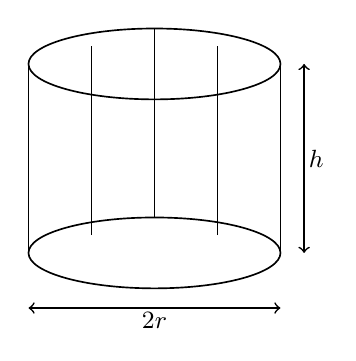
\begin{tikzpicture}[semithick, every node/.style={inner sep=1.4pt, font=\small}]
  % 下底椭圆
  \draw (0,0) ellipse (1.6 and 0.45);
  % 侧边
  \draw (-1.6,0) -- (-1.6,2.4);
  \draw (1.6,0) -- (1.6,2.4);
  % 上口（无上底面，只画椭圆口）
  \draw (0,2.4) ellipse (1.6 and 0.45);
  % 四条骨架竖线
  \draw (-1.6,0) -- (-1.6,2.4);
  \draw (-0.8,0.225) -- (-0.8,2.625);
  \draw (0,0.45) -- (0,2.85);
  \draw (0.8,0.225) -- (0.8,2.625);
  % 标注
  \draw[<->] (-1.6,-0.7) -- (1.6,-0.7);
  \node[below] at (0,-0.7) {$2r$};
  \draw[<->] (1.9,0) -- (1.9,2.4);
  \node[right] at (1.9,1.2) {$h$};
\end{tikzpicture}
\end{center}
\nopagebreak[4]
\Needspace{4\baselineskip}
\textbf{解析}

\Needspace{5\baselineskip}
（1）每个矩形骨架宽为 $2r$、高为 $h$，四个矩形共耗铁丝

\nopagebreak[4]
\[4\cdot2(2r+h)=9.6,\]

故 $2r+h=1.2$，$h=1.2-2r$。

\Needspace{5\baselineskip}
塑料片面积

\nopagebreak[4]
\[S=2\pi rh+\pi r^2
=2\pi r(1.2-2r)+\pi r^2
=2.4\pi r-3\pi r^2.\]

\nopagebreak[4]
\[S'=2.4\pi-6\pi r=0\Longrightarrow r=0.4.\]

\Needspace{5\baselineskip}
此时 $h=0.4$，

\nopagebreak[4]
\[S_{\max}=2.4\pi\cdot0.4-3\pi\cdot0.16
=0.48\pi\approx1.51.\]

（2）$r=0.3$ 时 $h=1.2-0.6=0.6$。正视图、侧视图均为 $0.6\times0.6$ 的矩形；俯视图为半径 $0.3$ 的圆（无上底面，圆内不画顶面轮廓）。

\gkanswer{答案：（1）$r=0.4$，$S_{\max}=0.48\pi\approx1.51$ 平方米；（2）三视图见解析。}

\end{answer}
\begin{answer}
\gksolhead{21}{}

\textbf{题目}：

已知数列 $\{a_n\}$ 的前 $n$ 项和为 $S_n$，且 $S_n=n-5a_n-85$，$n\in\mathbf N^*$．

（1）证明：$\{a_n-1\}$ 是等比数列；

（2）求数列 $\{S_n\}$ 的通项公式，并求出使得 $S_{n+1}>S_n$ 成立的最小正整数 $n$．

\Needspace{4\baselineskip}
\textbf{解析}

（1）$n=1$ 时 $a_1=S_1=1-5a_1-85$，得 $a_1=-14$。

\Needspace{5\baselineskip}
$n\geqslant2$ 时，

\nopagebreak[4]
\[a_n=S_n-S_{n-1}
=1-5a_n+5a_{n-1},\]

\nopagebreak[4]
\[6a_n=5a_{n-1}+1,\qquad a_n=\frac56a_{n-1}+\frac16.\]

\Needspace{5\baselineskip}
故

\nopagebreak[4]
\[a_n-1=\frac56(a_{n-1}-1),\]

且 $a_1-1=-15\neq0$，所以 $\{a_n-1\}$ 是首项 $-15$、公比 $\dfrac56$ 的等比数列。

\Needspace{5\baselineskip}
（2）由（1）

\nopagebreak[4]
\[a_n=1-15\left(\frac56\right)^{n-1},\]

\nopagebreak[4]
\[S_n=n-5a_n-85
=n-90+75\left(\frac56\right)^{n-1}.\]

\nopagebreak[4]
\[S_{n+1}-S_n=1+75\left[\left(\frac56\right)^n-\left(\frac56\right)^{n-1}\right]
=1-\frac{75}6\left(\frac56\right)^{n-1}.\]

\Needspace{5\baselineskip}
令其大于 $0$：

\nopagebreak[4]
\[\left(\frac56\right)^{n-1}<\frac6{75}=0.08.\]

$\left(\frac56\right)^{14}\approx0.0779<0.08$，$\left(\frac56\right)^{13}\approx0.0935>0.08$，故最小 $n-1=14$，即 $n=15$。

\gkanswer{答案：（1）证明见解析；（2）$S_n=n-90+75\left(\dfrac56\right)^{n-1}$，最小 $n=15$。}

\end{answer}
\begin{answer}
\gksolhead{22}{}

\textbf{题目}：

若实数 $x$、$y$、$m$ 满足 $|x-m|<|y-m|$，则称 $x$ 比 $y$ 接近 $m$．

（1）若 $x^2-1$ 比 $3$ 接近 $0$，求 $x$ 的取值范围；

（2）对任意两个不相等的正数 $a$、$b$，证明：$a^2b+ab^2$ 比 $a^3+b^3$ 接近 $2ab\sqrt{ab}$；

（3）已知函数 $f(x)$ 的定义域 $D=\{x\mid x\neq k\pi,\ k\in\mathbf Z,\ x\in\mathbf R\}$．任取 $x\in D$，$f(x)$ 等于 $1+\sin x$ 和 $1-\sin x$ 中接近 $0$ 的那个值．写出函数 $f(x)$ 的解析式，并指出它的奇偶性、最小正周期、最小值和单调性（结论不要求证明）．

\Needspace{4\baselineskip}
\textbf{解析}

\Needspace{5\baselineskip}
（1）$x^2-1$ 比 $3$ 接近 $0$：

\nopagebreak[4]
\[|x^2-1|<|3|=3,\qquad -2<x^2<4.\]

因 $x^2\geqslant0$，故 $x^2<4$，$x\in(-2,2)$。

\Needspace{5\baselineskip}
（2）令 $x=\sqrt a$，$y=\sqrt b$，$x\neq y$。则

\nopagebreak[4]
\[|a^2b+ab^2-2ab\sqrt{ab}|
=x^2y^2(x-y)^2,\]

\nopagebreak[4]
\[|a^3+b^3-2ab\sqrt{ab}|
=(x-y)^2(x^2+xy+y^2)^2.\]

\Needspace{5\baselineskip}
因 $x,y>0$，$x^2+xy+y^2>xy$，故

\nopagebreak[4]
\[x^2y^2<(x^2+xy+y^2)^2,\]

从而前者小于后者（$x\neq y$），命题成立。

\Needspace{5\baselineskip}
（3）比较 $|1+\sin x|$ 与 $|1-\sin x|$：当 $\sin x\geqslant0$ 时，$1-\sin x$ 更接近 $0$；当 $\sin x<0$ 时，$1+\sin x$ 更接近 $0$。故

\nopagebreak[4]
\[f(x)=1-|\sin x|.\]

它是偶函数，最小正周期 $\pi$，最小值 $0$；在 $\left(k\pi-\dfrac\pi2,k\pi\right)$ 上递减，在 $\left(k\pi,k\pi+\dfrac\pi2\right)$ 上递增（$k\in\mathbf Z$）。

\gkanswer{答案：（1）$(-2,2)$；（2）证明见解析；（3）$f(x)=1-\lvert\sin x\rvert$，偶函数、周期 $\pi$、最小值 $0$。}

\end{answer}
\begin{answer}
\gksolhead{23}{}

\textbf{题目}：

已知椭圆 $\Gamma$ 的方程为 $\dfrac{x^2}{a^2}+\dfrac{y^2}{b^2}=1$（$a>b>0$），$A(0,b)$、$B(0,-b)$ 和 $Q(a,0)$ 为 $\Gamma$ 的三个顶点．

（1）若点 $M$ 满足 $\overrightarrow{AM}=\dfrac12\left(\overrightarrow{AQ}+\overrightarrow{AB}\right)$，求点 $M$ 的坐标；

（2）设直线 $l_1:y=k_1x+p$ 交椭圆 $\Gamma$ 于 $C$、$D$ 两点，交直线 $l_2:y=k_2x$ 于点 $E$．若 $k_1\cdot k_2=-\dfrac{b^2}{a^2}$，证明：$E$ 为 $CD$ 的中点；

（3）设点 $P$ 在椭圆 $\Gamma$ 内且不在 $x$ 轴上，如何作过 $PQ$ 中点 $F$ 的直线 $l$，使得 $l$ 与椭圆 $\Gamma$ 两个交点 $P_1$、$P_2$ 满足 $\overrightarrow{PP_1}+\overrightarrow{PP_2}=\overrightarrow{PQ}$？令 $a=10$，$b=5$，点 $P$ 的坐标是 $(-8,-1)$．若椭圆 $\Gamma$ 上的点 $P_1$、$P_2$ 满足 $\overrightarrow{PP_1}+\overrightarrow{PP_2}=\overrightarrow{PQ}$，求点 $P_1$、$P_2$ 的坐标．

\Needspace{4\baselineskip}
\textbf{解析}

\Needspace{5\baselineskip}
（1）

\nopagebreak[4]
\[\overrightarrow{AM}=\frac12\left((a,-b)+(0,-2b)\right)
=\left(\frac a2,-\frac{3b}2\right),\]

\Needspace{5\baselineskip}
故

\nopagebreak[4]
\[M=A+\overrightarrow{AM}=\left(\frac a2,b-\frac{3b}2\right)
=\left(\frac a2,-\frac b2\right).\]

\Needspace{5\baselineskip}
（2）设 $C(x_1,y_1)$，$D(x_2,y_2)$。将 $y=k_1x+p$ 代入椭圆：

\nopagebreak[4]
\[\left(\frac1{a^2}+\frac{k_1^2}{b^2}\right)x^2
+\frac{2k_1p}{b^2}x+\frac{p^2}{b^2}-1=0.\]

\Needspace{5\baselineskip}
故

\nopagebreak[4]
\[x_E=\frac{x_1+x_2}{2}
=-\frac{k_1p/b^2}{1/a^2+k_1^2/b^2}
=-\frac{a^2k_1p}{b^2+a^2k_1^2}.\]

\Needspace{5\baselineskip}
又 $E$ 在 $l_2$ 上，$k_1x_E+p=k_2x_E$，故

\nopagebreak[4]
\[x_E=\frac{p}{k_2-k_1}.\]

利用 $k_1k_2=-\dfrac{b^2}{a^2}$ 可验证两式相等，故 $x_E=\dfrac{x_1+x_2}2$，即 $E$ 为 $CD$ 中点。

\Needspace{5\baselineskip}
（3）由 $\overrightarrow{PP_1}+\overrightarrow{PP_2}=\overrightarrow{PQ}$ 知 $F$ 为 $P_1P_2$ 的中点。椭圆 $\dfrac{x^2}{100}+\dfrac{y^2}{25}=1$ 中以 $F(x_0,y_0)$ 为中点的弦所在直线为

\nopagebreak[4]
\[\frac{xx_0}{100}+\frac{yy_0}{25}
=\frac{x_0^2}{100}+\frac{y_0^2}{25}.\]

\Needspace{5\baselineskip}
$P(-8,-1)$，$Q(10,0)$，故 $F(1,-\tfrac12)$。代入得

\nopagebreak[4]
\[\frac{x}{100}-\frac{y}{50}=0.02,\]

即 $l:x-2y=2$。

\Needspace{5\baselineskip}
与椭圆联立：

\nopagebreak[4]
\[x=2+2y,\qquad \frac{(2+2y)^2}{100}+\frac{y^2}{25}=1,\]

\nopagebreak[4]
\[y^2+y-12=0,\qquad y=3\ \text{\text{或}}\ -4.\]

故 $P_1(8,3)$，$P_2(-6,-4)$（或交换）。

\gkanswer{答案：（1）$\left(\dfrac a2,-\dfrac b2\right)$；（2）证明见解析；（3）$P_1(8,3)$，$P_2(-6,-4)$。}

\end{answer}